\documentclass[12pt]{article}
\usepackage[left=1cm, right=1cm, top=2cm,bottom=1.5cm]{geometry} 

\usepackage[parfill]{parskip}
\usepackage[utf8]{inputenc}
\usepackage[T2A]{fontenc}
\usepackage[russian]{babel}
\usepackage{enumitem}
\usepackage[normalem]{ulem}
\usepackage{amsfonts, amsmath, amsthm, amssymb, mathtools}
\usepackage{tabularx}
\usepackage{hhline}

\usepackage{accents}
\usepackage{fancyhdr}
\pagestyle{fancy}
\renewcommand{\headrulewidth}{1.5pt}
\renewcommand{\footrulewidth}{1pt}

\usepackage{graphicx}
\usepackage[figurename=Рис.]{caption}
\usepackage{subcaption}
\usepackage{float}

%%Наименование папки откуда забирать изображения
\graphicspath{ {./images/} }

%%Изменение формата для ввода доказательства
\renewcommand{\proofname}{$\square$  \nopunct}
\renewcommand\qedsymbol{$\blacksquare$}

%%Изменение отступа на таблицах
\addto\captionsrussian{%
	\renewcommand{\proofname}{$\square$ \nopunct}%
}
%% Римские цифры
\newcommand{\RN}[1]{%
	\textup{\uppercase\expandafter{\romannumeral#1}}%
}

%% Для удобства записи
\newcommand{\MR}{\mathbb{R}}
\newcommand{\MQ}{\mathbb{Q}}
\newcommand{\MI}{\mathrm{I}}
\newcommand{\MJ}{\mathrm{J}}
\newcommand{\MH}{\mathrm{H}}
\newcommand{\MT}{\mathrm{T}}
\newcommand{\MU}{\mathcal{U}}
\newcommand{\MV}{\mathcal{V}}
\newcommand{\VN}{\varnothing}
\newcommand{\VE}{\varepsilon}

\theoremstyle{definition}
\newtheorem{defn}{Опр:}
\newtheorem{rem}{Rm:}
\newtheorem{prop}{Утв.}
\newtheorem{exrc}{Упр.}
\newtheorem{lemma}{Лемма}
\newtheorem{theorem}{Теорема}
\newtheorem{corollary}{Следствие}

\newenvironment{cusdefn}[1]
{\renewcommand\thedefn{#1}\defn}
{\enddefn}

\DeclareRobustCommand{\divby}{%
	\mathrel{\text{\vbox{\baselineskip.65ex\lineskiplimit0pt\hbox{.}\hbox{.}\hbox{.}}}}%
}
%Короткий минус
\DeclareMathSymbol{\SMN}{\mathbin}{AMSa}{"39}

%Функция знака
\DeclareMathOperator{\sgn}{sgn}

%Обозначение константы
\DeclareMathOperator{\const}{\text{const}}

%Интеграл в большом формате
\DeclareMathOperator{\dint}{\displaystyle\int}

\newcommand{\smallerrel}[1]{\mathrel{\mathpalette\smallerrelaux{#1}}}
\newcommand{\smallerrelaux}[2]{\raisebox{.1ex}{\scalebox{.75}{$#1#2$}}}

\newcommand{\smallin}{\smallerrel{\in}}
\newcommand{\smallnotin}{\smallerrel{\notin}}

\newcommand*{\medcap}{\mathbin{\scalebox{1.25}{\ensuremath{\cap}}}}%
\newcommand*{\medcup}{\mathbin{\scalebox{1.25}{\ensuremath{\cup}}}}%

%Подпись символов снизу
\newcommand{\ubar}[1]{\underaccent{\bar}{#1}}

\begin{document}
\lhead{Математический анализ - \RN{2}}
\chead{Шапошников С.В.}
\rhead{Лекция - 1}
\section*{Неопределенный интеграл}
Пусть функция $f$ определена на интервале $(a,b)$.
\begin{defn}
	Дифференцируемая функция $F$ на интервале $(a,b)$ называется \uwave{первообразной} функции $f$, если: 
	$$
		F^\prime(x) = f(x), \, \forall x \in (a,b)
	$$
\end{defn}

\begin{prop}
	$F^\prime \equiv 0$ на $(a,b) \Leftrightarrow F = \const$.
\end{prop}
\begin{proof}\hfill\\
	$(\Leftarrow)$ Очевидно, $F = \const \Rightarrow F^\prime = 0$.
	
	$(\Rightarrow)$ По теореме Лагранжа: 
	$$
		F(x_1) - F(x_2) = F^\prime(c)(x_1 - x_2) = 0 \Rightarrow \forall x_1,x_2 \in (a,b), \, F(x_1) = F(x_2) \Rightarrow F(x) = \const
	$$
\end{proof}
\begin{rem}
	Важно, что определение идет на неразрывном интервале, в противном случае функция может быть кусочной и утверждение не будет верным.
\end{rem}

\begin{corollary}
	Если $F_1$ и $F_2$ - первообразные $f$ на $(a,b)$, то $F_1 - F_2 = \const$.
\end{corollary}
\begin{proof}
	$(F_1 - F_2)^\prime = f - f = 0 \Rightarrow$ используем предыдущее утверждение.
\end{proof}

Произвольную первообразную функции $f$ на $(a,b)$ обозначаем через $\dint f(x)\,dx$.

Если $F^\prime = f$, то $\dint f(x) \,dx = F + C$, где $C = \const$.
\begin{defn}
	Интеграл $\dint f(x)\,dx = F + C$, где $C = \const$ называется \uwave{неопределенным интегралом}. 
\end{defn}
\begin{defn}
	Процедура поиска первообразных называется \uwave{интегрированием}.
\end{defn}

\begin{rem}
	Почему такое обозначение? От английской буквы S (square).
\end{rem}

Пусть дана функция $f$, хотим найти $F\colon F^\prime = f$. По определению производной: 
$$
	F(a+h) - F(a) = f(a){\cdot}h + \underset{h \to 0}{\bar{o}(h)}, \quad \underset{h \to 0}{\bar{o}(h)}  = \alpha(a,h)h, \, \lim\limits_{h \to 0}\alpha(a,h) = 0
$$
Имея производную, мы знаем приращение функции при маленьких $h$: 
$$
	F(a+h) - F(a) \approx f(a){\cdot}h
$$
Поскольку мы ищем функцию $F$ с точностью до константы, возьмем точку $x_0$, зафиксируем там значение $F \colon F(x_0) = 0$, необходимо найти значение функции в точке $x$. Но $x$ расположен относительно далеко, а связь установлена на маленьких отрезках $\Rightarrow$ дробим отрезок $[x_0,x]$ на более мелкие отрезки.
\begin{figure}[H]
	\centering
	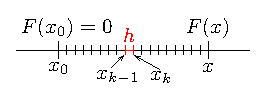
\includegraphics[width=0.25\textwidth]{1_1.eps}
	\caption{Нахождение значения в точке $x$ функции $F$.}
	\label{1_1}
\end{figure}
Таким образом на каждом маленьком отрезке мы можем написать: 
$$
	F(x_k) - F(x_{k-1}) \approx f(x_k)h, \; h = dx(h) \Rightarrow F(x_k) - F(x_{k-1}) \approx f(x_{k-1})h = f(x_{k-1})dx(h)
$$
Тогда выразим $F(x)$:
$$F(x) = \sum\limits_k \Big(F(x_k) - F(x_{k-1}) \Big) \approx \sum\limits_k f(x_{k-1})dx(h)$$
Поскольку равенство примерное, то оно становится точнее при $h \to 0 \Rightarrow$ сумма конечная превращается в сумму бесконечную: 
$$F(x) \approx \sum\limits_k f(x_{k-1})dx(h) \xrightarrow[h \to 0]{} \int f(x)\,dx$$

\begin{rem} Первообразная дифференциала $\neq$ дифференциал первообразной:
	\begin{enumerate}[label={(\arabic*)}]
		\item $\dint F^\prime(x)\,dx = \dint dF = F + C$;
		\item $d\bigg(\dint f(x)\,dx\bigg) = \bigg(\dint f(x)\,dx\bigg)^\prime dx = f(x) dx$;
	\end{enumerate}
\end{rem}

\section*{Свойства неопределнного интеграла}
Свойства неопределенных интегралов должны быть унаследованы от производных. Сравним свойства между ними:
\begin{enumerate}[label={(\arabic*)}]
	\item \textbf{\uwave{Линейность}}:
	
	\uline{Дифференцирование}: $(\alpha F + \beta G)^\prime = \alpha F^\prime + \beta G^\prime$;
	
	\uline{Интегрирование}: Пусть $F$ и $G$ - первообразные для $f$ и $g$ на $(a,b)$. Тогда $\alpha F + \beta G$ - первообразная для $\alpha f + \beta g$ на $(a,b)$, что записывается так:
	$$\int (\alpha f(x) + \beta g(x))\,dx = \alpha \int f(x) \, dx + \beta \int g(x) \, dx + C$$
	
	\item \textbf{\uwave{Правило Лейбница/Интегрирование по частям}}
	
	\uline{Дифференцирование}: $(F{\cdot}G)^\prime = F^\prime G + FG^\prime$;
	
	\uline{Интегрирование (\RN{1}-ый способ)}: Пусть $f$ и $g$ дифференцируемы на $(a,b)$ и у $f^\prime g$ есть первообразная, то у $fg^\prime$ тоже есть первообразная и верно равенство:
	$$\int (fg)^\prime \, dx = fg + C = \int f^\prime g \, dx + \int fg^\prime \, dx + C$$
	
	\uline{Интегрирование (\RN{2}-ый способ)}: $$\int f^\prime g \, dx = fg - \int fg^\prime \, dx + C$$
	\begin{proof}
		Поскольку $f$ и $g$ дифференцируемы, то по правилу Лейбница дифференцируемо их произведение $fg \Rightarrow$ первообразная $(fg)^\prime$ равна $fg \Rightarrow$ существует первообразная функции $fg^\prime$, так как эта функция равна: $(fg)^\prime - f^\prime g$ по правилу Лейбница. По свойству линейности у $(fg)^\prime - f^\prime g$ есть первообразная:
		$$\int fg^\prime \, dx = \int (fg)^\prime \, dx - \int f^\prime g \, dx + C = fg - \int f^\prime g \,dx + C$$ 
	\end{proof}
	
	\item \textbf{\uwave{Дифференцирование сложной функции/Замена переменной под интегралом}}
	
	\uline{Дифференцирование}: $(F(\varphi(t)))^\prime = F^\prime(\varphi(t)){\cdot} \varphi^\prime(t)$;
	
	\uline{Интегрирование}: Пусть $F$ - первообразная $f$ на $(a,b)$ и $\varphi\colon (\alpha, \beta) \to (a,b)$ - дифференцируема. Тогда $F(\varphi(t))$ - первообразная функции $f(\varphi(t)){\cdot}\varphi^\prime(t)$:
	$$\int f(\varphi(t)){\cdot}\varphi^\prime(t)\,dt = \int f(x) \, dx 
	\bigg\rvert_{x = \varphi(t)} + C = F(\varphi(t)) + C$$
	Мы знаем, что:
	$$\int f(\varphi(t)){\cdot}\underbrace{\varphi^\prime(t)\,dt}_{d\varphi} = \int f(\varphi)\, d \varphi$$
\end{enumerate}

\newpage
\section*{Таблица интегралов}
Рассматриваем те области определения, где функции определены и дифференцируемы. 

\begin{tabular}{|p{0.46\textwidth}|p{0.51\textwidth}|}	
	\hline
	\rule{0pt}{3ex}\textbf{Производные} &\textbf{Интегралы}\\[0.5ex] \hhline{|=|=|}
	\rule{0pt}{4.2ex}1) $f(x) = \const$; $(C)^\prime = (\const)^\prime = 0$;& 
	\rule{0pt}{4.2ex}1) $F(x) \equiv 0$; $\dint 0{\cdot}dx = \const = C$;
	\\[2.4ex]\hline
	\rule{0pt}{4.2ex}2) $f(x) = x^\alpha$; $(x^\alpha)^\prime = \alpha x^{\alpha - 1}$; & 
	\rule{0pt}{4.2ex}2) $F(x) = x^\alpha, \, \alpha \neq -1$;  $\dint x^\alpha \, dx = \dfrac{x^{\alpha + 1}}{\alpha + 1}  + C, \, \alpha \neq -1$;
	\\[2ex]\hline
	\rule{0pt}{4.2ex}3) $f(x) = \ln{|x|}$; $(\ln{|x|})^\prime = \dfrac{1}{x}$;& 
	\rule{0pt}{4.2ex}3) $F(x) = \dfrac{1}{x}$; $\dint \dfrac{1}{x} \, dx = \ln{|x|} + C$;
	\\[2ex]\hline
	\rule{0pt}{4.2ex}4) $f(x) = e^x$; $(e^x)^\prime = e^x$; & 
	\rule{0pt}{4.2ex}4) $F(x) = e^x$; $\dint e^x \, dx = e^x + C$;
	\\[2ex]\hline
	\rule{0pt}{4.2ex}5) $f(x) = \sin{x}$;  $(\sin{x})^\prime = \cos{x}$; & 
	\rule{0pt}{4.2ex}5) $F(x) = \cos{x}$; $\dint \cos{x} \, dx = \sin{x} + C$;
	\\[2ex]\hline
	\rule{0pt}{4.2ex}6) $f(x) = \cos{x}$;  $(\cos{x})^\prime = - \sin{x}$; & 
	\rule{0pt}{4.2ex}6) $F(x) = \sin{x}$; $\dint \sin{x} \, dx = -\cos{x} + C$;
	\\[2ex]\hline
	\rule{0pt}{4.2ex}7) $f(x) = \tg{x}$; $(\tg{x})^\prime = \dfrac{1}{\cos^2{x}}$; & 
	\rule{0pt}{4.2ex}7) $F(x) = \dfrac{1}{\cos^2{x}}$; $\dint \dfrac{1}{\cos^2{x}} \, dx = \tg{x} + C$;
	\\[2ex]\hline
	\rule{0pt}{4.2ex}8) $f(x) = \ctg{x}$; $(\ctg{x})^\prime = -\dfrac{1}{\sin^2{x}}$; & 
	\rule{0pt}{4.2ex}8) $F(x) = \dfrac{1}{\sin^2{x}}$; $\dint \dfrac{1}{\sin^2{x}} \, dx = - \ctg{x} + C$;
	\\[2ex]\hline
	\rule{0pt}{4.2ex}9) $f(x) = \arcsin{x}$; $(\arcsin{x})^\prime = \dfrac{1}{\sqrt{1-x^2}}$; & 
	\rule{0pt}{4.2ex}9) $F(x) = \dfrac{1}{\sqrt{1-x^2}}$; $\dint \dfrac{1}{\sqrt{1-x^2}} \, dx = \arcsin{x} + C$;
	\\[2ex]\hline
	\rule{0pt}{4.2ex}10) $f(x) = \arccos{x}$; $(\arccos{x})^\prime = -\dfrac{1}{\sqrt{1-x^2}}$; & 
	\rule{0pt}{4.2ex}10) $F(x) = \dfrac{1}{\sqrt{1-x^2}}$; $\dint \dfrac{1}{\sqrt{1-x^2}} \, dx = -\arccos{x} + C$;
	\\[2ex]\hline
	\rule{0pt}{4.2ex}11) $f(x) = \arctg{x}$; $(\arctg{x})^\prime = \dfrac{1}{1 + x^2}$; & 
	\rule{0pt}{4.2ex}11) $F(x) = \dfrac{1}{1 + x^2}$; $\dint \dfrac{1}{1 + x^2} \, dx = \arctg{x} + C$;
	\\[2ex]\hline
	\rule{0pt}{4.2ex}12) $f(x) = \arcctg{x}$; $(\arcctg{x})^\prime = -\dfrac{1}{1 + x^2}$; & 
	\rule{0pt}{4.2ex}12) $F(x) = \dfrac{1}{1 + x^2}$; $\dint \dfrac{1}{1 + x^2} \, dx = -\arcctg{x} + C$;
	\\[2ex]\hline
	
	\rule{0pt}{4.2ex}13) $f(x) = \ln\left(x+\sqrt{x^2\pm 1}\right)$; & 
	\rule{0pt}{4.2ex}13) $F(x) = \dfrac{1}{\sqrt{x^2\pm 1}}$; 
	\\[2ex]
	\vphantom{13)} $\left(\ln\left(x+\sqrt{x^2\pm 1}\right)\right)^\prime =\dfrac{1}{\sqrt{x^2\pm 1}}$; &
	\vphantom{13)} $\dint \dfrac{1}{\sqrt{x^2\pm 1}} \, dx = \ln\left(x+\sqrt{x^2\pm 1}\right) + C$;
	\\[2ex]\hline
	
	\rule{0pt}{4.2ex}14) $f(x) = \dfrac{1}{2}\ln \bigg|\dfrac{x-1}{x+1}\bigg|$; & 
	\rule{0pt}{4.2ex}14) $F(x) = \dfrac{1}{x^2-1}$; 
	\\[2ex]
	\vphantom{14)} $\left(\dfrac{1}{2}\ln \bigg|\dfrac{x-1}{x+1}\bigg|\right)^\prime =\dfrac{1}{2}\left(\dfrac{1}{x-1} - \dfrac{1}{x+1} \right) = \dfrac{1}{x^2-1}$; &
	\vphantom{14)} $\dint \dfrac{1}{x^2-1} \, dx = \dfrac{1}{2}\ln \bigg|\dfrac{x-1}{x+1}\bigg| + C$;
	\\[2ex]\hline
\end{tabular}

\newpage
\begin{defn}
	Назовем следующую функцию: $\ln\left(x+\sqrt{x^2\pm 1}\right)$ \uwave{длинным логарифмом}.
\end{defn}

\begin{defn}
	Назовем следующую функцию: $\dfrac{1}{2}\ln \bigg|\dfrac{x-1}{x+1}\bigg|$ \uwave{высоким логарифмом}.
\end{defn}

В некоторой степени можно сказать, что таблица интегралов $\Leftrightarrow$ таблица производных.

\begin{rem}
	Если область определения разбивается на несколько частей, то на каждой из них, при интегрировании, константа выбирается своя.
\end{rem}

\textbf{Пример}: $f(x) = x^{-2}$, для первообразной константы в положительной полуоси и в отрицательной - будут разными.

\begin{exrc}
	Решить уравнение $t = \ch{x} = \dfrac{e^x + e^{-x}}{2}$ (найти $x$).
\end{exrc}
\begin{proof}
	$$
		t =  \dfrac{e^x + e^{-x}}{2} \geq 0\Rightarrow 2t = e^x + e^{-x} \Rightarrow 2te^x = e^{2x} + 1 \Rightarrow e^{2x} - 2te^x + 1 =0 \Rightarrow e^x = \dfrac{2t \pm \sqrt{4t^2 - 4}}{2} \Rightarrow
	$$
	$$
		\Rightarrow e^x = t \pm \sqrt{t^2 - 1}, \, t \geq 0 \Rightarrow t^2 \geq 1 \Rightarrow t \geq 1 \Rightarrow t \pm \sqrt{t^2 - 1} > 0 \Rightarrow x = \ln\left(t \pm \sqrt{t^2 - 1}\right)
	$$
\end{proof}
\end{document}